\documentclass{article}
\usepackage{graphicx} % Required for inserting images
\usepackage[top=0.9in, bottom=1in, left=1.5in, right=1.5in]{geometry}
\usepackage[utf8]{inputenc}
\usepackage[icelandic]{babel}
\usepackage[T1]{fontenc}
\usepackage[sc]{mathpazo}
\usepackage[parfill]{parskip}
% Tables and lists
\usepackage{booktabs,tabularx}
\usepackage{multirow}
\usepackage{enumerate}
\usepackage{adjustbox}
\usepackage{multicol}
\usepackage{xcolor}
\usepackage{algpseudocode}
\usepackage{tikz}
\usetikzlibrary{arrows, positioning, calc}

% Math
\usepackage{amsmath, amsfonts, amssymb, amsthm}
% Graphics

\usepackage{graphicx}
\usepackage{tikz}
% Code environment
\usepackage{minted}
%\usepackage{bm}
%\usepackage{siunitx}
%\usepackage{animate}
%\usepackage{hyperref}
%\usepackage{movie15}
%\usepackage{multicol}
%\usepackage{changepage}
\title{Gagnasafnsfræði Verkefni 1}
\author{Ragnar Björn Ingvarsson, rbi3}


\begin{document}
	
	\maketitle
	
	\section{}
	
	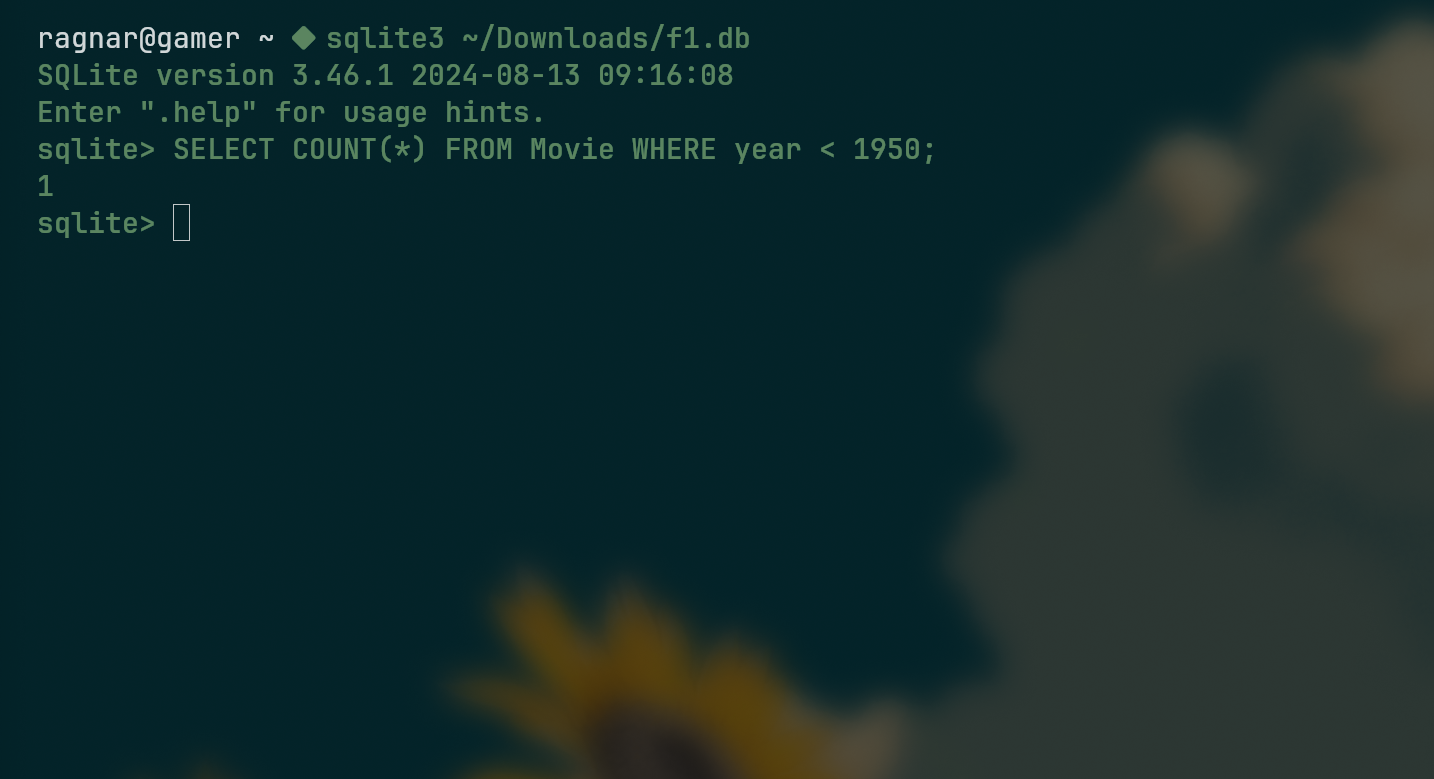
\includegraphics[scale=0.275]{sql.png}

	\section{}

	Gagnagrunnskerfi eru oft betri 
	fyrir stærri gagnagrunna og fyrirtæki sem þurfa að halda utan um mjög 
	víðfeng gögn og eru séræhæfð fyrir fyrirspurnir og síun á gögnum, en 
	Excel eða LibreOffice Calc eru erfið að skala upp til að passa 
	fyrir svoleiðis gagnagrunna. Hins vegar eru Excel og LibreOffice Calc 
	léttari og einfaldari fyrir fólk sem kann ekki á tækni nógu vel fyrir 
	t.d. SQL. Einnig hafa þau mun víðara notkunargildi þar sem þau geta 
	haldið utan um flókna reikninga, dagsetningar, o.fl.

	Svo í grunninn eru gagnasafnskerfi einmitt það, sérhæfð kerfi sem eiga 
	léttara með að halda utan um stór gagnasöfn og sía upplýsingar úr þeim 
	en töflureiknar eru einfaldari og með víðara notagildi 
	fyrir dagsdaglegt fólk.

\end{document}
